\documentclass[a4paper]{article}
\usepackage{tkz-euclide}
\usetkzobj{all} 

%% ================== commands ==========================
\newcommand{\myShowPoints}[2]{
\tkzDrawPoints(#1) \tkzLabelPoints[#2](#1)
}		

\newcommand{\myGetMidPoint}[3]{
\tkzDefMidPoint(#1,#2)\tkzGetPoint{#3}
}		
%% ------------------ end of commands -------------------


\usepackage{enumerate}
\begin{document}


\section{Points} % (fold)
\label{sec:points}
\begin{enumerate}
	\item Define a point with specific coordinates 
	\begin{figure}[h]
	\centering
		\begin{tikzpicture}
			\tkzDefPoint(0,0){A}
			\tkzDefPoint(1,1){B}
			% \tkzDrawPoints(A,B)
			% \tkzLabelPoints(A,B)
			\myShowPoints{A,B}{above}
		\end{tikzpicture}
	\end{figure}
\end{enumerate}

% section points (end)


\section{Lines, Segments} % (fold)
\label{sec:lines_segments}
\begin{enumerate}
	\item Draw a segment between two points
	\begin{figure}[h]
	\centering
		\begin{tikzpicture}
			\tkzDefPoint(0,0){A}
			\tkzDefPoint(1,5){B}
			\tkzDrawSegment(A,B)
			% \tkzDefMidPoint(A,B)\tkzGetPoint{M}
			\myGetMidPoint{A}{B}{M}
			% mid point 
			% \tkzDrawPoints(M)\tkzLabelPoints(M)
			\myShowPoints{A,B,M}{left}


		\end{tikzpicture}
	\end{figure}


	\item Intersections of two lines
		\begin{figure}[h]
		\centering
		\begin{tikzpicture}
			% define points 
			\tkzDefPoint(0,0){A}
			\tkzDefPoint(1,5){B}
			\tkzDefPoint(-1,4){C}
			\tkzDefPoint(6,0){D}
			% line segments
			\tkzDrawSegment(A,B)
			\tkzDrawSegment(C,D)
			% intersection
			\tkzInterLL(A,B)(C,D) \tkzGetPoint{I}
			%show points
			\myShowPoints{A,B,C,D}{left}
			\myShowPoints{I}{above right}
			% \tkzDrawPoint[color = red](I)

			
		\end{tikzpicture}
	\end{figure}

	\item Orthogonal and Parallel
	\begin{figure}[h]
	\centering
		\begin{tikzpicture}
			\tkzDefPoint(-3,0){A}
			\tkzDefPoints{0/1/B, -2/2/C, 1/-2/D}
			\tkzDrawLines[add = 0.1 and .1](C,D)
			%% orthogonal
			\tkzDefLine[orthogonal=through A](C,D)
		  	\tkzInterLL(C,D)(A,tkzPointResult) \tkzGetPoint{H}
		  	\tkzDrawSegments(A,H)
		  	\tkzMarkRightAngle[fill=gray!10](A,H,D)
		  	%% parallel 
			\tkzDefLine[parallel=through B](C,D)
		  	\tkzDrawLine[add = .5 and -.2](B,tkzPointResult)

			\myShowPoints{B,D}{right}
			\myShowPoints{A,C,H}{left}
\end{tikzpicture}
	\end{figure}

\end{enumerate}
% section lines_segments (end)

\section{Triangles} % (fold)
\label{sec:triangles}
\begin{itemize}
	\item Given three points, draw the triangle
	\begin{figure}[h]
	\centering
		\begin{tikzpicture}
			\tkzDefPoint(0,0){A}
			\tkzDefPoint(1,5){B}
			\tkzDefPoint(-1,4){C}
			
			\tkzDrawPolygon(A,B,C)

		\end{tikzpicture}
	\end{figure}

\end{itemize}


% section triangles (end)

\section{Circles} % (fold)
\label{sec:circles}

% section circles (end)

% \begin{tikzpicture}
% \tkzDefPoint(1,2){A}
% \tkzDefPoint(3,4){B}
% \tkzDefPoint(2,4){C}
% \tkzDrawArc[ultra thick, blue](O,C)(A)

% \end{tikzpicture}
 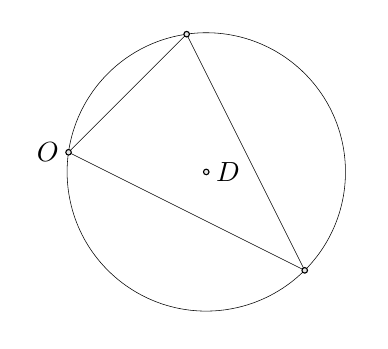
\begin{tikzpicture}[scale=1.5]
	\tkzDefPoint(0,0){O}
	\tkzDefPoint(2,-1){A}
	\tkzDefPoint(1,1){B}
	% \tkzDrawArc[color=blue](O,A)(B)
	% \tkzDrawArc[color=green](O,B)(A)
	\tkzDrawLines[add = 0 and 0](O,A O,B A,B)
	\tkzCircumCenter(A,B,O)\tkzGetPoint{D}
	% \tkzDrawArc(O,B)(A)
	\tkzDrawArc(D,B)(A)
	\tkzDrawArc(D,A)(B)
	\tkzDrawPoints(O,A,B)
	% \tkzLabelPoints[below](O,A,B)
	\tkzLabelPoints[left](O)
	\tkzDrawPoints(D)
	\tkzLabelPoints[right](D)


 \end{tikzpicture}

\end{document}